\documentclass[11pt]{article}
\usepackage[utf8]{inputenc}
\usepackage[a4paper,margin=1in]{geometry}
\usepackage{hyperref}
\usepackage{listings}
\usepackage{graphicx}
\usepackage{color}
\usepackage{float}
\usepackage{enumitem}
\usepackage{booktabs}
\usepackage{tikz}
\usepackage{minted}
\usepackage{fancyhdr}

% Define colors for different sections
\definecolor{sectioncolor}{RGB}{70,130,180}
\definecolor{subsectioncolor}{RGB}{0,100,0}

\definecolor{codegreen}{rgb}{0,0.6,0}
\definecolor{codegray}{rgb}{0.5,0.5,0.5}
\definecolor{codepurple}{rgb}{0.58,0,0.82}

\lstdefinestyle{mystyle}{
    commentstyle=\color{codegreen},
    keywordstyle=\color{magenta},
    numberstyle=\tiny\color{codegray},
    stringstyle=\color{codepurple},
    basicstyle=\ttfamily\footnotesize,
    breakatwhitespace=false,         
    breaklines=true,                 
    captionpos=b,                    
    keepspaces=true,                 
    numbers=left,                    
    numbersep=5pt,                  
    showspaces=false,                
    showstringspaces=false,
    showtabs=false,                  
    tabsize=2
}

\lstset{style=mystyle}

\title{Knowledge Graph with Personality Traits\\Implementation Details}
\author{Technical Documentation}
\date{\today}

\begin{document}

\pagestyle{fancy}
\fancyhf{}
\rhead{Knowledge Graph with Personality Traits}
\lhead{Technical Documentation}
\rfoot{Page \thepage}

\maketitle

\begin{abstract}
This document presents a comprehensive implementation of a Knowledge Graph system that combines entity extraction, relationship mapping, and personality trait analysis. The system processes textual input to create an interactive graph visualization that captures both factual relationships and personality characteristics of entities mentioned in the text.
\end{abstract}

\tableofcontents
\newpage

\section{Introduction}
\subsection{Project Overview}
This document describes the implementation of a Knowledge Graph (KG) system that extracts entities and their relationships from text, while also modeling personality traits. The system combines Natural Language Processing (NLP) techniques with graph-based representation and personality trait analysis.

\section{System Architecture}

\subsection{Core Components}
The system consists of three main components:
\begin{itemize}
    \item Knowledge Graph Builder (KGBuilder)
    \item Personality Trait Estimator
    \item Visualization Engine
\end{itemize}

\section{Project Overview and Architecture}
This knowledge graph system integrates natural language processing with personality trait analysis to create a comprehensive representation of entities and their relationships in text data.

\subsection{System Architecture}
Figure 1 shows the high-level architecture of the system:

\begin{figure}[H]
    \centering
    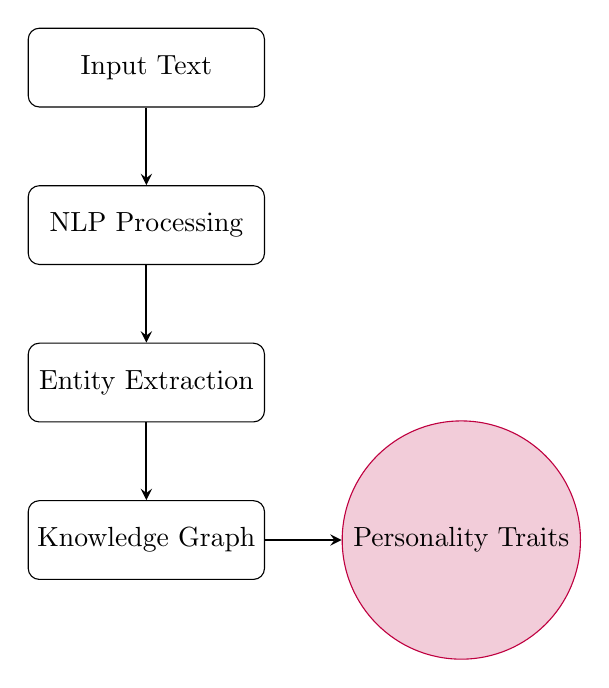
\begin{tikzpicture}[node distance=2cm]
% Define styles
\tikzstyle{entity} = [rectangle, rounded corners, minimum width=3cm, minimum height=1cm, text centered, draw=black]
\tikzstyle{trait} = [circle, draw=purple, fill=purple!20, minimum size=1.5cm]
\tikzstyle{arrow} = [thick,->,>=stealth]

% Draw nodes
\node (text) [entity] {Input Text};
\node (nlp) [entity, below of=text] {NLP Processing};
\node (entities) [entity, below of=nlp] {Entity Extraction};
\node (kg) [entity, below of=entities] {Knowledge Graph};
\node (personality) [trait, right of=kg, xshift=2cm] {Personality Traits};

% Draw arrows
\draw [arrow] (text) -- (nlp);
\draw [arrow] (nlp) -- (entities);
\draw [arrow] (entities) -- (kg);
\draw [arrow] (kg) -- (personality);

\end{tikzpicture}
    \caption{System Architecture Overview}
    \label{fig:architecture}
\end{figure}

\section{Technical Implementation}

\subsection{Knowledge Graph Construction}
The knowledge graph is built through several sophisticated steps:

\begin{enumerate}[label=\textbf{\arabic*.}, itemsep=0.5em]
    \item \textbf{Text Processing:}
    \begin{itemize}
        \item Uses spaCy's advanced NLP pipeline
        \item Handles co-reference resolution
        \item Performs sentence segmentation and tokenization
    \end{itemize}
    
    \item \textbf{Entity Extraction:}
    \begin{itemize}
        \item Identifies PERSON, ORG, SKILL, and TRAIT entities
        \item Uses custom entity patterns for domain-specific recognition
        \item Maintains entity context for relationship inference
    \end{itemize}
    
    \item \textbf{Relationship Detection:}
    \begin{itemize}
        \item Analyzes syntactic dependencies
        \item Infers semantic relationships
        \item Maps entity connections based on context
    \end{itemize}
    
    \item \textbf{Personality Integration:}
    \begin{itemize}
        \item Implements Big Five personality model
        \item Calculates trait scores (0-1 range)
        \item Associates traits with relevant entities
    \end{itemize}
\end{enumerate}

\subsection{Code Organization}
The project follows a modular structure:

\begin{lstlisting}[language=Python, caption=Project Structure]
src/
  kg_personality/
    kg_builder.py      # Core graph construction
    personality.py     # Trait analysis
    data_generator.py  # Synthetic data creation
data/                 # Example datasets
tests/               # Comprehensive test suite
documentation/       # Technical documentation
\end{lstlisting}

\section{Core Components}

\subsection{Entity Recognition System}
The system recognizes and processes various entity types:

\begin{table}[H]
\centering
\begin{tabular}{@{}llp{8cm}@{}}
\toprule
\textbf{Entity Type} & \textbf{Example} & \textbf{Description} \\
\midrule
PERSON & "Sarah Chen" & Individual names and mentions \\
ORG & "TechLab" & Organizations and institutions \\
SKILL & "Python" & Technical abilities and competencies \\
TRAIT & "analytical" & Personality characteristics \\
\bottomrule
\end{tabular}
\caption{Entity Types and Examples}
\label{tab:entities}
\end{table}

\subsection{Personality Modeling}
The system implements the Big Five personality framework:

\begin{itemize}[label=$\bullet$]
    \item \textbf{Openness:} Curiosity and creativity
    \item \textbf{Conscientiousness:} Organization and responsibility
    \item \textbf{Extraversion:} Social interaction and energy
    \item \textbf{Agreeableness:} Cooperation and empathy
    \item \textbf{Neuroticism:} Emotional stability and anxiety
\end{itemize}

\section{Implementation Examples}

\subsection{Basic Usage}
Here's a complete example of using the system:

\begin{lstlisting}[language=Python, caption=Basic Usage Example]
from kg_personality.kg_builder import KGBuilder
from kg_personality.personality import PersonalityEstimator

# Initialize components
kg = KGBuilder()
pe = PersonalityEstimator()

# Process text and build graph
text = """
Sarah Chen is a creative and analytical researcher at TechLab.
She excels in Python and machine learning.
"""
G = kg.build_from_text(text, source_id="doc")

# Extract entities and add personality
entities = [n for n in G.nodes() if n.startswith("doc_ent_")]
personality = pe.estimate_for_entities(entities)
kg.merge_personality(G, personality)

# Add relationships
kg.add_relationships()

# Generate visualization
kg.export_to_html("knowledge_graph.html")
\end{lstlisting}

\subsection{Visualization Features}
The visualization system provides:

\begin{itemize}
    \item Interactive node exploration
    \item Color-coded entity types
    \item Relationship indicators
    \item Personality trait tooltips
    \item Zoom and pan controls
\end{itemize}

\section{Testing and Validation}

\subsection{Test Coverage}
The project includes comprehensive tests:

\begin{enumerate}
    \item Entity extraction accuracy
    \item Relationship inference
    \item Personality trait calculation
    \item Graph construction validation
    \item Visualization generation
\end{enumerate}

\subsection{Performance Considerations}
Key performance aspects:

\begin{itemize}
    \item Efficient graph operations using NetworkX
    \item Optimized NLP pipeline with spaCy
    \item Scalable visualization with pyvis
    \item Memory-efficient data structures
\end{itemize}

\section{Future Enhancements}
Planned improvements include:

\begin{enumerate}
    \item \textbf{Advanced NLP Features:}
    \begin{itemize}
        \item Enhanced co-reference resolution
        \item Sentiment analysis integration
        \item Temporal relationship tracking
    \end{itemize}
    
    \item \textbf{Visualization Enhancements:}
    \begin{itemize}
        \item Custom layout algorithms
        \item Advanced filtering options
        \item Interactive graph editing
    \end{itemize}
    
    \item \textbf{API Integration:}
    \begin{itemize}
        \item Real LLM integration (e.g., OpenAI)
        \item REST API endpoints
        \item Streaming data support
    \end{itemize}
\end{enumerate}

\section{Conclusion}
This implementation demonstrates the successful integration of knowledge graphs with personality trait analysis, providing a foundation for advanced text analytics and relationship modeling. The system's modular design and comprehensive documentation facilitate future extensions and improvements.

\end{document}